\chapter{소리, 양자 조화진동자, 그리고 제2법칙}

\lectureoverview{제2법칙이 도달할 지점이지만, 그에 앞서 구체적인 계산 두 가지를 살펴본다. 음속을 통해 열역학적 미분량이 어떻게 관측 가능한 운동으로 나타나는지 확인한다. 이어서 조화진동자로 강성이 큰 자유도에 고전적 등분배 법칙이 적용되지 않는다는 점을 살펴보고, 양자역학이 모드를 하나씩 활성화하는 방식도 확인한다. 마지막으로 위상 공간 흐름, 거친 묘사, 혼돈, 재귀를 이용해 가역적인 미시적 동역학과 증가하는 엔트로피 사이의 겉보기 모순으로 돌아간다. 이를 통해 제2법칙은 예외 없는 역학적 금지가 아니라 압도적으로 높은 확률로 성립하는 법칙임을 밝힌다.}

\section{제2법칙에 관한 약속}

핵심 문제는 말로 표현하기는 쉽지만 설명하기는 어렵다. 뉴턴 역학 방정식은 가역적이다. 어떤 미시적 과정이 허용된다면 그 시간을 거꾸로 한 과정도 허용된다. 그런데도 제2법칙은 거시적 과정에 엔트로피가 보통 증가한다는 특징으로 규정되는 선호 방향이 있다고 말한다. 이 긴장 관계를 살펴보겠지만, 바로 시작하지는 않겠다. 먼저 통계역학이 구체적인 정보를 어떻게 산출하는지 확인한 다음, 고전물리학이 양자물리학으로 대체되도록 만든 역사적 수수께끼를 간단한 계산에서 마주하는 편이 낫다.

첫 번째 예는 수치로 답을 구하되 의도적으로 거칠게 근사한다. 희박 기체의 음속을 추정해 보자. 두 번째 예는 가정이 주어진 범위에서 정확히 계산한다. 열저장고에 놓인 조화진동자의 평균 에너지를 구한다. 이 진동자를 통해 등분배 법칙에서 양자화된 에너지 준위로, 하나의 모드에서 무한히 많은 모드로 나아간 뒤, 다입자계가 초기 상태를 잊는다는 말의 의미를 묻는 문제로 돌아온다.

\section{음속의 분자 규모}

희박 기체에 작은 과밀 영역이 있다고 생각해 보자. 분자들이 밀집된 곳에서 빠져나가면서 이 영역은 퍼져 나가므로, 그 전파 속도는 분자 속도와 비슷한 규모일 것이다. 등분배 법칙으로 분자 하나의 운동에너지를 구하면 다음과 같다.
\begin{equation}
 \frac{3}{2}k_B T
 =\frac{1}{2}m\expect{v^2},
 \qquad
 \expect{v^2}=\frac{3k_B T}{m}.
 \label{eq:sm7-molecular-speed}
\end{equation}
여기서 온도는 절대영도를 기준으로 측정하며, 실험실 단위를 쓰기 위해 \(k_B\)를 다시 포함했다. 이 논증은 규모만 추정한다. 분자의 제곱평균제곱근 속도가 집단적인 음파의 속도 자체인 것은 아니다.

좀 더 체계적으로 유도하려면 기체의 작은 요소를 생각한다. 서로 마주 보는 면에 작용하는 압력이 다르면 알짜힘이 생기며, 그 가속도는 질량 밀도에 반비례한다. 그 결과는 다음 형태를 띤다.
\begin{equation}
 c_s^2=
 \left(\frac{\partial P}{\partial \rho_m}\right)_{\cal C},
 \qquad
 \rho_m=m\rho,
 \label{eq:sm7-sound-general}
\end{equation}
여기서 \(\rho\)는 수밀도이고, 아래첨자 \({\cal C}\)는 교란이 따르는 열역학적 조건을 지정한다. 판서에서 계산한 식은 다음과 같다.
\begin{equation}
 P=\rho k_B T
 \quad\Longrightarrow\quad
 \frac{1}{m}
 \left(\frac{\partial P}{\partial\rho}\right)_T
 =\frac{k_B T}{m}.
 \label{eq:sm7-sound-isothermal}
\end{equation}
이는 등온 음속 추정식이다. 제곱한 음속은 \eqref{eq:sm7-molecular-speed}의  \(3\)배이고, 음속은 \(\sqrt{3}\)배만큼 차이가 난다.

\begin{figure}[t]
\centering
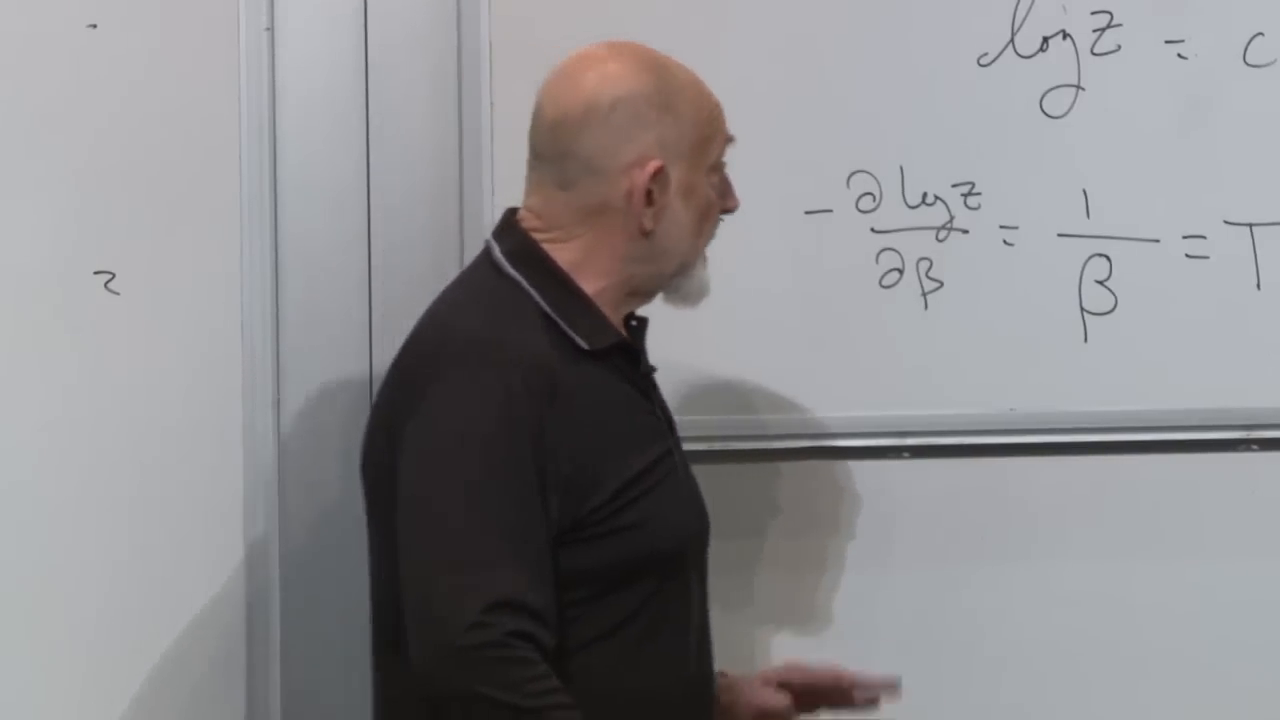
\includegraphics[width=0.90\textwidth]{lecture_07_figure_02.png}
\caption{분자 속도 추정, 압력 미분, 이상기체 대입식을 함께 나타냈다.}
\lectureframe{00:08:55}
\end{figure}

여기에는 중요한 보완이 필요하다. 진폭이 작은 음파는 보통 이웃한 기체 요소 사이에 열이 흐르는 것보다 빠르게 기체를 압축하고 팽창시킨다. 따라서 국소적인 운동은 등온이 아니라 대략 단열적이다.
\begin{equation}
 c_s^2=
 \left(\frac{\partial P}{\partial\rho_m}\right)_S.
 \label{eq:sm7-sound-adiabatic}
\end{equation}
단열지수가 \(\gamma\)인 이상기체에서는
\begin{equation}
 P\rho_m^{-\gamma}=\text{constant},
 \qquad
 c_s^2=\gamma\frac{P}{\rho_m}
       =\gamma\frac{k_B T}{m}.
 \label{eq:sm7-sound-ideal-adiabatic}
\end{equation}
실온의 이원자 기체인 공기는 \(\gamma\simeq 7/5\)이다. 그러므로 온도를 고정한 계산은 유용한 첫 추정치이고, 단열 미분이 물리적으로 적절한 보정을 제공한다.

대략적인 값으로
\begin{equation}
\begin{aligned}
 k_B&\simeq1.3\times10^{-23}\ {\rm J\,K^{-1}},
 &T&\simeq300\ {\rm K},\\
 m_{\rm air}&\simeq4\times10^{-26}\ {\rm kg}.&&
\end{aligned}
 \label{eq:sm7-air-data}
\end{equation}
분자 속도를 추정하면 약 \(500\ {\rm m\,s^{-1}}\)이다. 여기서 온도는 화씨처럼 기준점에서 벗어난 척도가 아니라 켈빈 단위의 절대온도여야 한다. 익숙한 음속은 대략 \(300\ {\rm m\,s^{-1}}\) 규모이며, 이상기체에 대한 단열식으로 계산하면 실온에서 약 \(340\ {\rm m\,s^{-1}}\)이다. 따라서 이 거친 계산으로도 올바른 물리적 규모를 얻었다.

\begin{figure}[t]
\centering
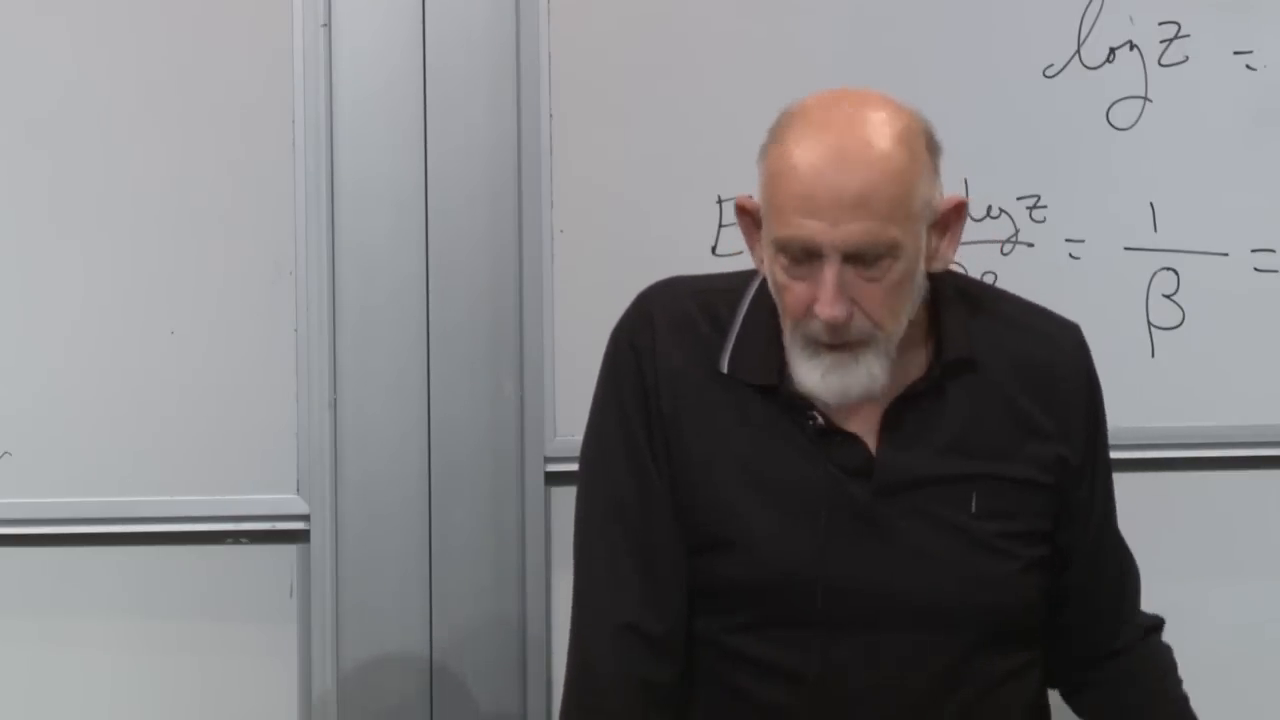
\includegraphics[width=0.90\textwidth]{lecture_07_figure_03.png}
\caption{볼츠만 상수, 양성자 질량의 약 \(30\)배인 유효 분자 질량, 그리고 \(T\simeq300\ {\rm K}\)를 사용한 실온 공기의 음속 추정.}
\lectureframe{00:10:55}
\end{figure}

미시적인 설명이 가능해지기 훨씬 전에도 압력을 밀도의 함수로 측정하면 음속을 구할 수 있었다. 통계역학적 논증은 그 결과로 얻는 거시적 속도가 개별 분자의 열속도로 정해진다는 놀라운 해석을 더해 준다.

\begin{classroomqa}
\audiencequestion{분자 질량에 중성자도 더해야 하나요? 질소에 대한 수 \(14\)는 양성자만 세나요?}
\lecturerresponse{인용된 원자량에는 이미 양성자와 중성자가 모두 포함되어 있다. 분자 질소는 원자량이 약 \(14\)인 원자 두 개로 이루어져 있으므로, 질량은 양성자 질량의 약 \(28\)배이다. 이 추정에는 \(28\)을 \(30\)로 반올림해도 충분하다.
\lecturetimestamp{00:10:58--00:11:16}}
\end{classroomqa}

\begin{classroomqa}
\audiencequestion{계수 \(3\)는 병진 방향이 세 개라는 데서 나왔는데, 음파는 한 방향으로 전파됩니다. 그러면 계수 \(3\)를 없애야 하나요?}
\lecturerresponse{이 질문은 3차원 제곱평균제곱근 분자 속도를 1차원 전파 속도와 동일시하면 안 된다는 점을 올바르게 짚는다. 도입부의 논증은 규모만 파악하려는 설명이었다. 제어된 답은 압력 미분과 파동에 적절한 열역학적 조건에서 얻는다.
\lecturetimestamp{00:11:12--00:12:00}}
\end{classroomqa}

\begin{classroomqa}
\audiencequestion{파동이 진행되는 동안 온도가 일정하다고 가정하고 미분한 건가요?}
\lecturerresponse{판서에 나온 이상기체 대입식에서는 그렇게 했다. 아주 작은 교란에서는 온도를 일정하게 두는 것이 그럴듯한 잠정 추정일 수 있다. 표준적인 보정은 일반적인 음파가 대략 단열적이라는 점을 반영하며, 이때 등온 미분 대신 \(\left(\partial P/\partial\rho_m\right)_S\)를 사용한다.
\lecturetimestamp{00:12:59--00:14:01}}
\end{classroomqa}

\begin{classroomqa}
\audiencequestion{압력 변화와 밀도 변화가 모두 작다면, 그 미분값도 작아지나요?}
\lecturerresponse{아니다. 미분은 무한소 극한에서 두 작은 변화량의 비다. \(\delta P\)와 \(\delta\rho\)는 모두 작을 수 있지만, \(\delta P/\delta\rho\)는 유한한 값으로 남아 파동 속도를 정한다.
\lecturetimestamp{00:14:03--00:14:23}}
\end{classroomqa}

\begin{classroomqa}
\audiencequestion{기체에서 액체나 고체로 갈 때처럼 기체를 압축하면 음속도 높아져야 하나요?}
\lecturerresponse{그렇다. 미분값은 고려 중인 상태에서 계산하며, \(P(\rho,T)\)가 계속 선형일 필요는 없다. 분자들이 서로 가까이 압축되면 상태방정식은 비이상적이 되고 \(\partial P/\partial\rho\)는 크게 증가할 수 있다.
\lecturetimestamp{00:14:25--00:15:13}}
\end{classroomqa}

\begin{classroomqa}
\audiencequestion{모든 압력에서 \(500\ {\rm m\,s^{-1}}\)를 사용할 수 있나요?}
\lecturerresponse{아니다. 이 값은 이상기체 방정식이 유용한 근사인 저밀도 범위에 해당한다. \(P(\rho,T)\)에 밀도의 고차항이 포함되기 시작하면 미분값과 음속은 압력과 밀도에 따라 달라진다.
\lecturetimestamp{00:15:14--00:16:29}}
\end{classroomqa}

\begin{classroomqa}
\audiencequestion{음파가 대략 분자 속도로 퍼진다는 처음의 그림도 밀도가 증가하면 성립하지 않나요?}
\lecturerresponse{그럴 가능성이 크다. 그 그림은 희박 기체에 맞춘 것이다. 밀도가 높아지면 집단적 상호작용이 점점 중요해지는데, 바로 그런 이유로 상태방정식의 미분값이 더 일반적인 설명이 된다.
\lecturetimestamp{00:16:32--00:16:53}}
\end{classroomqa}

\begin{classroomqa}
\audiencequestion{질소 분자의 질량을 \(30\)이 아니라 대략 \(28\) 양성자 질량이라고 쓴 이유는 무엇인가요?}
\lecturerresponse{이 추정에 필요한 수치 정밀도만 있으면 되므로 \(28\)를 \(30\)으로 반올림했다. 처음의 \(500\ {\rm m\,s^{-1}}\) 추정값을 \(\sqrt{3}\simeq1.7\)로 나누어도 \(300\ {\rm m\,s^{-1}}\)에 가까워지지만, 보정값을 제어된 방식으로 계산하려면 단열 미분을 써야 한다.
\lecturetimestamp{00:16:54--00:17:27}}
\end{classroomqa}

\section{열저장고 속 고전 조화진동자 하나}

이제 자유롭게 병진하는 분자 대신 조화진동자 하나를 두고 나머지는 모두 열저장고로 취급한다. 스프링에 매달린 질량이 바로 떠오르는 그림이지만, 이 모형은 훨씬 폭넓게 적용된다. 전자기 공동의 모드는 진동하고, 결정 속 원자들도 진동한다. 평형에서 조금 벗어난 거의 모든 안정한 계는 1차 근사에서 조화운동을 한다.

평형 위치에서 측정한 변위를 \(x\), 운동량을 \(p\), 질량을 \(m\), 스프링 상수를 \(\kappa\)라 하면 해밀토니안은 다음과 같다.
\begin{equation}
 H(x,p)=\frac{p^2}{2m}+\frac{\kappa x^2}{2},
 \qquad
 \omega=\sqrt{\frac{\kappa}{m}}.
 \label{eq:sm7-classical-hamiltonian}
\end{equation}
열저장고가 \(T\)를 정하며, 여기서부터는 다시 \(k_B=1\)로 두므로 \(\beta=1/T\)이다. 방 안에 둔 진동자는 약 \(300\ {\rm K}\)의 온도에 도달하고, 액체 헬륨에 담긴 진동자의 온도는 몇 켈빈에 불과하다. 태양 중심에 스프링을 놓는다면 스프링으로 남아 있지 못하겠지만, 이 예는 환경의 역할을 분명하게 보여 준다. 볼츠만 가중치는 다음처럼 인수분해된다.
\begin{equation}
 e^{-\beta H}
 =e^{-\beta p^2/(2m)}
  e^{-\beta\kappa x^2/2}.
 \label{eq:sm7-factorized-weight}
\end{equation}

\begin{figure}[t]
\centering
\includegraphics[width=0.90\textwidth]{lecture_07_figure_04.png}
\caption{스프링에 매달린 질량으로 나타낸 진동자와 운동에너지 및 퍼텐셜 에너지의 합으로 이루어진 해밀토니안.}
\lectureframe{00:20:55}
\end{figure}

자유 기체와 달리, 위치 적분은 용기의 부피만을 주지 않는다. 복원 퍼텐셜이 각 변위에 가중치를 부여한다.
\begin{equation}
 Z_{\rm cl}
 =\frac{1}{h}\int_{-\infty}^{\infty}dp
             \int_{-\infty}^{\infty}dx\,
 e^{-\beta p^2/(2m)}
 e^{-\beta\kappa x^2/2}.
 \label{eq:sm7-classical-z}
\end{equation}
인수 \(1/h\)는 1차원 고전 분배함수를 무차원으로 만든다. 판서 계산에서는 이 인수가 \(\beta\)와 무관하고 평균 에너지에 영향을 주지 않으므로 생략했다.

\begin{figure}[t]
\centering
\includegraphics[width=0.90\textwidth]{lecture_07_figure_05.png}
\caption{운동량과 변위에 관한 가우스 적분으로 분리한 고전 진동자 분배함수.}
\lectureframe{00:22:55}
\end{figure}

운동량 적분에서는 다음과 같이 치환한다.
\begin{equation}
 q=\sqrt{\frac{\beta}{2m}}\,p,
 \qquad
 dp=\sqrt{\frac{2m}{\beta}}\,dq.
 \label{eq:sm7-p-gaussian-substitution}
\end{equation}
위치 적분에서는 다음과 같이 치환한다.
\begin{equation}
 y=\sqrt{\frac{\beta\kappa}{2}}\,x,
 \qquad
 dx=\sqrt{\frac{2}{\beta\kappa}}\,dy.
 \label{eq:sm7-x-gaussian-substitution}
\end{equation}
\(\int_{-\infty}^{\infty}e^{-u^2}\,du=\sqrt{\pi}\)이므로, 판서에서 사용한 정규화 전 위상 공간 적분은 다음과 같다.
\begin{equation}
 \int dp\,dx\,e^{-\beta H}
 =\frac{2\pi}{\beta}\sqrt{\frac{m}{\kappa}}
 =\frac{2\pi}{\beta\omega}.
 \label{eq:sm7-classical-z-unnormalized}
\end{equation}
위상 공간 셀을 다시 포함하면
\begin{equation}
 Z_{\rm cl}=\frac{2\pi}{h\beta\omega}
           =\frac{1}{\beta\hbar\omega}.
 \label{eq:sm7-classical-z-normalized}
\end{equation}

에너지에는 \(\beta\)에 대한 의존성만 중요하다.
\begin{equation}
 \begin{aligned}
 \log Z_{\rm cl}&=\text{constant}-\log\beta,\\
 \expect{H}
 &=-\frac{\partial\log Z_{\rm cl}}{\partial\beta}\\
 &=\frac{1}{\beta}=T.
 \end{aligned}
 \label{eq:sm7-classical-energy}
\end{equation}

\begin{figure}[t]
\centering
\includegraphics[width=0.90\textwidth]{lecture_07_figure_06.png}
\caption{오른쪽 칠판의 고전 계산 전체 과정: 가우스 인수분해, \(Z\propto(\beta\omega)^{-1}\), 그리고 \(\expect{H}=1/\beta=T\).}
\lectureframe{00:30:15}
\end{figure}

공간 진동자가 하나이므로 \(3\) 인수는 없다. 서로 독립인 이차항이 두 개이므로 \(1/2\) 인수도 남지 않는다. 각 가우스 적분은 \(T/2\)를 기여한다.
\begin{equation}
 \expect{K}=\frac{T}{2},
 \qquad
 \expect{U}=\frac{T}{2},
 \qquad
 \expect{H}=T.
 \label{eq:sm7-equipartition-oscillator}
\end{equation}
이는 가장 유용한 형태의 등분배 법칙이다. 고전 해밀토니안의 독립적인 이차항마다 \(T/2\)가 기여한다.

답은 \(m\)와 \(\kappa\) 모두에 의존하지 않는다. 하지만 운동 자체는 이 매개변수들에 따라 달라진다.
\begin{equation}
 \expect{p^2}=mT,
 \qquad
 \expect{x^2}=\frac{T}{\kappa},
 \qquad
 \expect{\dot{x}^2}=\frac{T}{m}.
 \label{eq:sm7-classical-fluctuations}
\end{equation}
따라서 질량이 클수록 더 느리게 움직이고 스프링이 더 뻣뻣할수록 진폭이 작아지지만, 평균 에너지는 여전히 \(T\)이다. \(\kappa\)가 엄청나게 커지면 이 결과는 곤혹스러워진다. 너무 뻣뻣해서 움직이지 않는 스프링은 얼어붙은 구속조건처럼 보여야 할 텐데, 고전적 등분배 법칙은 여전히 그 에너지를 \(T\)로 준다.

\begin{classroomqa}
\audiencequestion{\(\kappa\to\infty\)일 때 분배함수는 0으로 간다. 그런데 어떻게 그 로그를 계속 사용할 수 있나요?}
\lecturerresponse{\(\kappa\)를 유한하지만 임의로 큰 값으로 두면 된다. 그것은 \(\log Z\)에 상수항으로 더해지고 \(\beta\)와 무관하므로 \(\beta\)에 대한 미분으로 여전히 \(T\)를 얻는다. 극한에서 생기는 불편함은 실제다. 고전적 계산은 내부적으로 일관되지만, 매우 뻣뻣한 진동자에 필요한 자연의 특성을 빠뜨리고 있다.
\lecturetimestamp{00:34:01--00:34:54}}
\end{classroomqa}

\begin{classroomqa}
\audiencequestion{이상기체의 분배함수에는 \(N!\)가 필요했습니다. 여기에도 비슷한 계승 인수가 있어야 하나요?}
\lecturerresponse{아니다. 여기서는 지정된 진동자 하나를 다루며, \(N\)개의 동일한 입자를 서로 바꾸어 세는 것이 아니다. 서로 독립인 모드가 여러 개라면 분배함수들을 곱한다. 비구별성 인수는 다른 셈 문제에 해당한다.
\lecturetimestamp{00:35:03--00:35:40}}
\end{classroomqa}

\section{고전적 등분배 법칙이 위기를 맞은 이유}

실제 분자는 구조가 없는 점이 아니다. 이원자 분자는 진동할 수 있는 결합을 가지므로 내부 진동자가 있다. 고전적인 방식으로 단순하게 세면 보통 온도에서도 그 모드에 추가적인 열에너지를 배정하게 된다. 의도적으로 개략화한 계산에서 진동자 하나를 활성화하면 에너지는 \(3T/2\)에서 \(5T/2\) 쪽으로 증가한다. 정확한 열용량 계산에는 회전 자유도도 포함해야 하고, 에너지와 그 온도 미분값도 구별해야 한다. 결정적인 실험 사실은 더 단순하다. 고전적 등분배 법칙의 예측과 달리, 강성이 큰 내부 모드는 저온에서 기여하지 않았다.

분자에 내부 구조가 없다고 할 수도 있겠지만, 이는 터무니없다. 아니면 고전역학에 빠진 요소가 있음을 인정해야 한다. 그 요소가 양자역학이다. 여기서는 양자역학의 아주 적은 부분만 필요하다. 조화진동자의 에너지 준위 간격이 일정하다는 사실뿐이다.

\section{양자 조화진동자}

먼저 에너지 기준점을 옮겨 들뜬 상태의 스펙트럼을 다음과 같이 쓴다.
\begin{equation}
 E_n^{\rm exc}=n\hbar\omega,
 \qquad n=0,1,2,\ldots.
 \label{eq:sm7-shifted-spectrum}
\end{equation}
이제 분배함수는 위상 공간 적분이 아니라 실제 합으로 주어진다.
\begin{align}
 Z_{\rm exc}
 &=\sum_{n=0}^{\infty}e^{-\beta n\hbar\omega} \notag\\
 &=1+x+x^2+\cdots
  =\frac{1}{1-x},
 \qquad x=e^{-\beta\hbar\omega}, \notag\\
 &=\frac{1}{1-e^{-\beta\hbar\omega}}.
 \label{eq:sm7-quantum-z}
\end{align}

\begin{figure}[t]
\centering
\includegraphics[width=0.90\textwidth]{lecture_07_figure_07.png}
\caption{등간격 에너지 준위와 양자 조화진동자 분배함수의 등비급수 계산.}
\lectureframe{00:42:05}
\end{figure}

미분하면 평균 들뜬 에너지를 얻는다.
\begin{align}
 E_{\rm exc}
 &=-\frac{\partial\log Z_{\rm exc}}{\partial\beta}
  =-\frac{1}{Z_{\rm exc}}
    \frac{\partial Z_{\rm exc}}{\partial\beta}
 \notag\\
 &=\hbar\omega\,
   \frac{e^{-\beta\hbar\omega}}
        {1-e^{-\beta\hbar\omega}}
  =\frac{\hbar\omega}{e^{\beta\hbar\omega}-1}.
 \label{eq:sm7-quantum-energy}
\end{align}

\begin{figure}[t]
\centering
\includegraphics[width=0.90\textwidth]{lecture_07_figure_08.png}
\caption{양자 분배함수를 \(\beta\)에 대해 미분해 구한 열적 들뜬 에너지.}
\lectureframe{00:46:05}
\end{figure}

\subsection{고온}

\(\beta\hbar\omega\ll1\)일 때,
\begin{equation}
 e^{-\beta\hbar\omega}
 =1-\beta\hbar\omega
  +O\!\left((\beta\hbar\omega)^2\right).
 \label{eq:sm7-high-t-expansion}
\end{equation}
\eqref{eq:sm7-quantum-energy}의 분자는 \(\hbar\omega\)에 가까워지고, 분모는 선도항에서 \(\beta\hbar\omega\)이다. 따라서
\begin{equation}
 E_{\rm exc}\simeq\frac{1}{\beta}=T.
 \label{eq:sm7-high-t-energy}
\end{equation}
열에너지 범위 안에 여러 에너지 준위 간격이 들어갈 때 양자적 결과는 고전적 등분배 법칙을 회복한다.

\subsection{저온}

\(\beta\hbar\omega\gg1\)일 때 지수항은 매우 작다.
\begin{equation}
 E_{\rm exc}
 \simeq\hbar\omega e^{-\beta\hbar\omega}.
 \label{eq:sm7-low-t-energy}
\end{equation}
진동자의 열적 들뜸은 지수적으로 억제된다. 에너지를 옮겨 쓴 관례에서는 거의 0이며, 물리적인 영점 에너지는 아래에서 다시 포함한다.

\begin{figure}[t]
\centering
\includegraphics[width=0.90\textwidth]{lecture_07_figure_09.png}
\caption{저온 전개: 첫 번째 열적 들뜸이 \(e^{-\beta\hbar\omega}\)만큼 억제된다.}
\lectureframe{00:51:55}
\end{figure}

교차는 다음 조건에서 일어난다.
\begin{equation}
 \beta\hbar\omega\sim1,
 \qquad\text{or equivalently}\qquad
 T\sim\hbar\omega.
 \label{eq:sm7-crossover}
\end{equation}
이 조건에는 직접적인 의미가 있다. 고전적 등분배 법칙은 진동자 에너지가 \(T\)라고 예측한다. 그 규모가 하나의 에너지 준위 간격보다 작아지면 양자 효과를 무시할 수 없게 된다. 따라서
\begin{equation}
\begin{aligned}
 \hbar\omega\gg T&:\quad \text{frozen and quantum},\\
 \hbar\omega\ll T&:\quad \text{active and classical}.
\end{aligned}
 \label{eq:sm7-regimes}
\end{equation}
더 뻣뻣한 스프링은 \(\omega=\sqrt{\kappa/m}\)가 더 크므로 고전적으로 거동하기 시작하려면 온도가 더 높아야 한다.

\section{물질을 가열하면 자유도가 나타난다}

저온에서 이원자 분자는 결합의 진동이 강성이 커서 얼어붙어 있으므로 점입자처럼 열적 거동을 보일 수 있다. \(T\)가 \(\hbar\omega\)을 지나 높아지면 진동 모드가 활성화된다. 회전 모드는 더 낮은 온도 규모에서 활성화될 수 있으며, 온도가 더 높아지면 다른 내부 운동이 드러나고 마침내 원자가 이온화된다. 가열은 고정된 모드 목록에 에너지를 더하기만 하는 것이 아니다. 낮은 온도에서는 보이지 않던 자유도를 드러낸다.

가상의 중첩 분자를 생각하면 요점이 더 분명해진다. 두 원자가 뻣뻣한 스프링으로 연결되어 있고, 겉으로 보이는 원자 하나도 더 뻣뻣한 스프링으로 연결된 원자 두 개로 이루어져 있다. 낮은 \(T\)에서는 두 구조 모두 점처럼 보인다. 첫 번째 임계점에서 바깥쪽 진동이 나타나고, 두 번째 임계점에서 안쪽 구조가 드러난다. 계의 복잡성은 에너지 규모에 따라 하나씩 밝혀진다.

\begin{classroomqa}
\audiencequestion{진동자가 이미 고전적 영역에 들어선 뒤에도 더 가열하면 스프링이 더 뻣뻣해지거나 진동수가 바뀌나요?}
\lecturerresponse{아니다. 스프링 상수와 진동수는 그대로다. 온도가 높아지면 전형적인 운동량과 진폭이 커져 에너지가 증가한다. 강성은 고전 법칙이 적용되기 시작하는 온도를 정할 뿐, 온도에 따라 스프링이 더 뻣뻣해지는 것은 아니다.
\lecturetimestamp{01:03:17--01:05:11}}
\end{classroomqa}

\subsection{결정과 아인슈타인의 비열}

결정에는 매우 많은 진동 모드가 있다. 고전적 등분배 법칙은 활성화된 각 진동자에 \(T\) 규모의 에너지를 배정하므로 저온 비열을 과대평가한다. 아인슈타인의 1907 모형은 결정 진동을 양자역학적으로 다루어 열에너지가 준위 간격에 이를 때까지 진동이 억제되는 이유를 보였다. 더 정밀한 고체 모형은 다양한 진동수 분포를 고려하지만, 동결 원리는 이미 아인슈타인의 계산에 담겨 있다.

\begin{classroomqa}
\audiencequestion{아인슈타인이 노벨상을 받은 업적이 이것인가요? 양자역학이 확립된 뒤에야 이 연구를 했나요?}
\lecturerresponse{아니다. 노벨상 수상 이유는 광전 효과였다. 비열 모형은 양자역학의 완전한 기초가 이해되기 훨씬 전인 1907에 발표되었다. 아인슈타인은 중요한 양자 개념을 받아들이고 발전시켰지만, 훗날 성숙한 이론의 일부 측면에는 반대했다.
\lecturetimestamp{00:58:38--01:03:16}}
\end{classroomqa}

\begin{classroomqa}
\audiencequestion{고전 통계역학은 이산 상태의 합을 위치와 운동량에 대한 겉보기에 균일한 적분으로 바꾸었습니다. 이러한 상태 세기를 정당화하는 근거는 무엇인가요?}
\lecturerresponse{궁극적인 근거는 양자역학에서 나온다. 고온 극한에서는
\[
 Z_{\rm exc}\simeq\frac{1}{\beta\hbar\omega},
\]
이는 무차원 고전 결과인 \eqref{eq:sm7-classical-z-normalized}와 정확히 일치한다. 에너지 준위 간격을 분해해 볼 수 없게 되면 위상 공간의 양자 셀이 고전적인 위상 공간 측도로 이어진다.
\lecturetimestamp{00:59:38--01:03:06}}
\end{classroomqa}

\subsection{현에는 무한히 많은 진동자가 들어 있다}

바이올린이나 기타 줄은 기본 진동, 더 높은 배음, 그리고 점점 더 짧은 파장의 정상 모드들로 분해된다. 수학적으로 진동자 모드는 무한히 많다. 고전적 등분배 법칙이 각 모드에 \(T\)의 에너지를 배정한다면 열평형에 있는 줄의 에너지는 무한대가 된다. 양자역학은 이 재앙을 막는다. 파장이 가장 짧은 모드의 진동수가 가장 높아 유한한 온도에서는 계속 얼어붙어 있고, \(T\)가 높아질수록 모드가 점차 더 많이 활성화된다. 같은 논리가 나중에 흑체 복사의 기초가 된다.

\begin{figure}[t]
\centering
\includegraphics[width=0.90\textwidth]{lecture_07_figure_10.png}
\caption{줄 위에 중첩된 여러 정상 모드. 연속적인 줄이 조화진동자 무한 개의 모음인 이유를 보여 준다.}
\lectureframe{01:09:30}
\end{figure}

\begin{classroomqa}
\audiencequestion{양자에서 고전으로의 교차를 직접 관측할 수 있나요? 가열하면 저온에서 보이던 거동이 뒤집히나요?}
\lecturerresponse{그렇다. 결정의 비열이 온도에 따라 변하는 양상을 측정하면 진동 모드의 동결과 이후의 활성화를 뚜렷하게 관측할 수 있다.
\lecturetimestamp{01:09:11--01:10:13}}
\end{classroomqa}

\begin{classroomqa}
\audiencequestion{진동자가 여러 개일 때는 각 모드마다 단일 진동자 분배함수를 반복해서 쓰나요?}
\lecturerresponse{독립 모드들의 경우
\[
\begin{aligned}
 Z_{\rm tot}&=\prod_j Z_j,&
 \log Z_{\rm tot}&=\sum_j\log Z_j,\\
 E_{\rm tot}&=\sum_j E_j.&&
\end{aligned}
\]
\(\hbar\omega_j\gg T\)인 모드는 열적 기여가 지수적으로 작고, 임계값보다 낮은 모드는 상당한 기여를 한다.
\lecturetimestamp{01:10:14--01:11:00}}
\end{classroomqa}

\begin{classroomqa}
\audiencequestion{진동자의 영점 에너지 \(\hbar\omega/2\)는 어떻게 되었나요?}
\lecturerresponse{물리적인 에너지 준위는 다음과 같다.
\[
 E_n=\left(n+\frac12\right)\hbar\omega.
\]
따라서
\[
 \begin{aligned}
 Z_{\rm phys}
 &=e^{-\beta\hbar\omega/2}Z_{\rm exc},\\
 E_{\rm phys}
 &=\frac{\hbar\omega}{2}
  +\frac{\hbar\omega}{e^{\beta\hbar\omega}-1}.
 \end{aligned}
\]
공통된 에너지 이동은 준위 확률, 엔트로피, 열용량, 열적 들뜬 에너지를 바꾸지 않지만 절대 평균 에너지를 \(\hbar\omega/2\)만큼 이동시킨다. \(Z\)의 곱셈 인자는 \(\beta\)에 의존하므로 절대 에너지를 구할 때는 버리면 안 된다.
\lecturetimestamp{01:11:08--01:11:37}}
\end{classroomqa}

\section{가역성 수수께끼로서의 제2법칙}

이제 앞서 약속한 문제로 돌아가자. 제2법칙에 따르면 일반적인 거시적 시간 변화는 비가역적이며 엔트로피는 증가하는 경향이 있다. 미시적 해밀토니안 시간 변화는 가역적이다. 가역적인 정확한 상태의 사상이 어떻게 거시적 상태에 대한 비가역 법칙을 낳을 수 있을까?

계를 고차원 위상 공간의 한 점으로 나타내자.
\[
 \Gamma=(q_1,\ldots,q_N,p_1,\ldots,p_N).
\]
우리가 아는 상태는 보통 정확한 한 점이 아니다. 부피가 \(\Omega_A\)인 유계 영역 \(A\)에서 확률밀도가 균일하다고 하자.
\begin{equation}
 f(\Gamma)=
 \begin{cases}
  1/\Omega_A,&\Gamma\in A,\\
  0,&\Gamma\notin A.
 \end{cases}
 \label{eq:sm7-uniform-blob}
\end{equation}
\(k_B=1\)인 단위계에서 미시적으로 분해된 깁스 엔트로피는 다음과 같다.
\begin{equation}
 S_{\rm fine}
 =-\int d\Gamma\,f\log f
 =\log\Omega_A.
 \label{eq:sm7-blob-entropy}
\end{equation}
영역이 작을수록 정보가 많고 엔트로피는 낮다. 따라서 부호는 분명하다. 불확실성이 커지면 점유된 영역이 넓어지고 \(\log\Omega_A\)도 증가한다.

\begin{figure}[t]
\centering
\includegraphics[width=0.90\textwidth]{lecture_07_figure_11.png}
\caption{전체 위치-운동량 위상 공간을 도식적으로 2차원으로 잘라 본 곳에 표시한 유계 확률 영역.}
\lectureframe{01:20:20}
\end{figure}

\begin{classroomqa}
\audiencequestion{계는 그려진 영역 안에 물리적으로 갇혀 있나요? 이미 평형 상태인가요?}
\lecturerresponse{아니다. 이 영역은 초기 상태에 대해 알고 있는 내용을 나타낼 뿐, 위상 공간의 벽이 아니다. 평형 분포일 필요도 없다. 예를 들어 방 한쪽 구석의 탱크에 처음 갇혀 있는 기체는 특별한 비평형 정보를 보여 준다.
\lecturetimestamp{01:14:55--01:15:24}}
\end{classroomqa}

\section{리우빌 흐름과 거친 묘사에서의 증가}

리우빌 정리에 따르면 해밀토니안 흐름은 위상 공간 부피를 보존한다. 정확한 영역은 이동하고 늘어나고 접히며 극도로 얇아질 수 있지만
\begin{equation}
 \Omega_{A(t)}=\Omega_{A(0)},
 \qquad
 S_{\rm fine}(t)=S_{\rm fine}(0).
 \label{eq:sm7-liouville}
\end{equation}
이산적인 대응물은 상태의 가역 순열이다. 처음에 주사위가 두 상태 중 하나에 있다고 알고 있다면, 일대일 시간 변화로 그 두 상태가 다른 두 상태로 바뀔 수는 있지만 가능한 상태의 수는 달라지지 않는다.

실제 묘사에는 유한한 분해능만 있다. 양자역학은 자연스러운 위상 공간 셀을 제공하며, 고전 실험도 양자 이론을 끌어들이지 않아도 측정 능력이 유한하다. 해밀토니안 흐름에 따라 영역은 길고 가느다란 뱀 모양이 될 수 있다. 이웃한 주름 사이의 간격이 분해능보다 작아지면, 구분할 수 없는 이웃 영역을 하나의 거친 셀로 대체한다. 정확한 점유 부피는 그대로지만 거친 셀들의 합집합은 커진다.
\begin{equation}
 \Omega_{\rm coarse}(t)\geq\Omega_{A(t)},
 \qquad
 S_{\rm coarse}(t)=\log\Omega_{\rm coarse}(t).
 \label{eq:sm7-coarse-entropy}
\end{equation}

\begin{figure}[t]
\centering
\includegraphics[width=0.90\textwidth]{lecture_07_figure_12.png}
\caption{유한한 분해능의 셀로 본 부피 보존 필라멘트. 정확한 검은 필라멘트의 면적은 그대로지만, 빨간색 거친 셀은 더 큰 유효 영역을 차지한다.}
\lectureframe{01:22:10}
\end{figure}

\begin{classroomqa}
\audiencequestion{거친 셀들이 겹치는데, 리우빌 정리에 어긋나지 않나요?}
\lecturerresponse{아니다. 리우빌 정리는 일대일 대응과 부피 보존을 유지하는 정확한 필라멘트에 적용된다. 겹침은 흐릿한 묘사에서 생긴다. 상태가 어느 가느다란 가닥에 있는지에 관한 정보를 버린 것이다.
\lecturetimestamp{01:21:32--01:21:50}}
\end{classroomqa}

솜에 비유하면 이해하기 쉽다. 섬유를 모두 합한 물질의 부피는 거의 그대로여도, 솜을 풀어 놓으면 각각의 섬유를 분해해 볼 수 없는 관찰자에게는 더 큰 부피를 차지하는 것처럼 보인다. 마찬가지로 위상 공간의 영역은 점점 더 미세한 촉수를 뻗고, 그 촉수는 또 더 미세한 촉수를 만든다. 고정된 유한 분해능으로는 결국 그 구조를 따라갈 수 없다.

\begin{classroomqa}
\audiencequestion{고전역학에서는 엔트로피 증가가 단지 그렇게 보일 뿐이고, 양자역학이 근본적인 분해능 한계를 부과해 그 증가를 실제로 만드는 건가요?}
\lecturerresponse{거친 묘사에 관한 논증에는 양자역학적 한계가 필요하지 않다. 엔트로피는 계와 그 묘사에서 유지되는 거시적 구분을 함께 가리킨다. 무한한 미시 정보가 있다면 미시적으로 분해된 엔트로피는 일정하다. 고정된 유한 분해능에서는 혼돈으로 생긴 필라멘트가 결국 구분되지 않게 되고 거친 묘사의 엔트로피가 증가한다.
\lecturetimestamp{01:24:04--01:25:20}}
\end{classroomqa}

\section{혼돈, 유한한 접근 가능 영역, 그리고 평형화}

상자 속 기체의 위치는 제한되어 있다. 전체 에너지가 순간적으로 한 입자에 집중되더라도, 유한한 전체 에너지에서는 운동량 역시 제한된다. 따라서 통상적인 구속 조건 아래에서 동역학적으로 접근 가능한 에너지 껍질의 측도는 유한하다.

\begin{figure}[t]
\centering
\includegraphics[width=0.90\textwidth]{lecture_07_figure_13.png}
\caption{필라멘트와 그 거친 묘사 옆에 나타낸 유계 접근 가능 위상 공간 영역.}
\lectureframe{01:28:10}
\end{figure}

혼돈계에서는 서로 가까운 초기점들이 한동안 비슷한 이력을 따르다가 서로 멀어진다. 당구에서 큐볼의 방향이 눈에 띄지 않을 만큼 조금 달라지면 그 차이가 뒤이은 충돌에 전달된다. 차이는 누적되어 마지막 상태들은 서로 무관해진다. 따라서 초기 상태의 한 영역 전체가 접근 가능한 영역을 따라 늘어나고 접힌다. 유한한 해상도에서는 넓고 거의 균일한 평형 기술에 가까워진다.

\begin{figure}[t]
\centering
\includegraphics[width=0.90\textwidth]{lecture_07_figure_14.png}
\caption{제한된 접근 가능 영역을 따라 하나의 간결한 특수 상태가 복잡한 필라멘트로 진화하는 동안, 조대화된 셀들은 훨씬 더 넓은 영역으로 퍼졌다.}
\lectureframe{01:33:10}
\end{figure}

두 가지 단서를 염두에 두어야 한다. 혼돈이라는 사실만으로 모든 궤적이 접근 가능한 모든 근방을 방문한다고 증명되는 것은 아니다. 그런 더 강한 표본화 주장을 하려면 에르고딕성이나 혼합성이 필요하다. 또한 모든 물리계가 혼돈계인 것도 아니다. 일반적인 다체 기체와 이상화된 당구는 여기서 의도하는 사례이며, 이런 계에서는 혼합성이 유용한 물리적 기대가 된다.

\section{재귀가 비가역성을 없애지는 않는다}

모든 공기 분자가 특별히 준비된 속도 패턴을 지닌 채 방 한구석에서 출발한다고 하자. 충돌이 일어나면 분자들은 빠르게 방 전체로 퍼지고, 조대화된 기술은 평형에 도달한다. 유한한 측도 보존 위상공간에서 푸앵카레 재귀 정리는 거의 모든 초기점이 출발점에 임의로 가까운 곳으로 돌아온다고 말한다. 허용오차 \(\epsilon>0\)에 대해 재귀 시간 \(t_R(\epsilon)\)은 이 정리의 가정 아래 유한하지만, 거시계에서는 터무니없이 길다. 무한히 정밀한 점으로 정확히 돌아올 필요도 없고, 일반적으로 그렇게 되리라 기대하지도 않는다.

\begin{classroomqa}
\audiencequestion{당구의 예에서 큐볼을 치면 에너지가 들어가 고립된 계의 진화라는 가정이 깨지지 않나요?}
\lecturerresponse{선택한 초기 상태는 공을 친 직후부터 시작하며, 그때의 에너지는 이미 포함되어 있다. 재귀는 그 뒤에 이어지는 고립된 이상화 당구의 동역학을 다룬다. 초기 상태에 가까운 상태로 돌아온다는 것은 선택한 허용오차 안에서 큐볼이 랙에 다가가는 것과 동등한 배치를 포함한다.
\lecturetimestamp{01:35:37--01:35:55}}
\end{classroomqa}

\begin{classroomqa}
\audiencequestion{기체가 결국 구석으로 돌아올 수 있다면, 정보가 사라진 것이고 계는 정말 가역적인가요?}
\lecturerresponse{미시적 동역학은 처음부터 끝까지 가역적이다. 미세한 상관관계를 더는 분해해 보지 않기 때문에 조대화된 엔트로피가 증가할 수 있지만, 극히 드문 요동으로 계가 특수한 초기 거시상태에 가까이 돌아올 수도 있다. 따라서 재귀와 조대화된 비가역성은 양립한다.
\lecturetimestamp{01:37:34--01:38:15}}
\end{classroomqa}

이로써 볼츠만의 핵심적인 정식화에 이른다. 논리적으로 가능한 모든 순간에 엔트로피가 증가하는 것은 아니다. 큰 계가 비평형 거시상태에 있을 때, 그 상태와 양립하는 미시적 후속 상태 가운데 훨씬 더 많은 경우가 더 특수한 상태가 아니라 더 큰 거시상태로 향한다. 엔트로피는 \emph{아마도} 증가한다. 엔트로피가 감소하는 요동과 재귀도 허용되지만, 그 확률과 시간 척도는 일상적인 거시적 경험에서 보이지 않을 만큼 작고 길다. 가역성 문제는 통계역학의 역사에서 큰 논쟁거리였으며 볼츠만에게도 큰 부담이었다. 그렇다고 이 역사적 연관성을 그의 삶에 대한 단순한 인과적 주장으로 바꾸어서는 안 된다.

\section{혼돈이 뜻하는 것}

혼돈을 좀 더 조작적으로 정의해 보자. 초기 위상점 두 개가 \(\delta\Gamma(0)\)만큼 다르다고 하자. 혼돈 방향에서는 선형화된 분리가 의미 있는 영역에서 보통 다음 관계가 성립한다.
\begin{equation}
 \lVert\delta\Gamma(t)\rVert
 \sim e^{\lambda t}\lVert\delta\Gamma(0)\rVert,
 \qquad \lambda>0,
 \label{eq:sm7-lyapunov-growth}
\end{equation}
수 \(\lambda\)를 리아푸노프 지수라고 한다. 시간 \(t\) 동안 예측하려면 초기 자료를 대략 \(e^{-\lambda t}\)에 비례하는 정밀도로 알아야 한다. 동역학 법칙의 정밀도도 중요하다. 초기 조건의 오차와 함께 모형의 오차도 증폭된다. 날씨가 익숙한 예다.

\begin{classroomqa}
\audiencequestion{\emph{대부분}의 계가 혼돈계라는 원리가 있나요, 아니면 단지 경험적 사실인가요?}
\lecturerresponse{혼돈 해밀토니안과 비혼돈 해밀토니안은 각각 무한히 많다. 게다가 \emph{대부분}이라는 말을 쓰려면 해밀토니안들의 공간에 측도를 정의해야 한다. 복잡하게 상호작용하는 계는 혼돈계인 경우가 많지만, 모든 해밀토니안을 보고 즉시 분류할 수 있는 간단하고 보편적인 검사는 없다.
\lecturetimestamp{01:39:27--01:40:49}}
\end{classroomqa}

\begin{classroomqa}
\audiencequestion{이 논의에서 \emph{혼돈적}이라는 말은 정확히 무엇을 뜻하나요?}
\lecturerresponse{가까운 위상 궤적들이 충분히 빠르게 분리되므로, 긴 시간 뒤를 예측하려면 초기 조건에 대한 지식을 지수적으로 더 정밀하게 알아야 한다. 조화진동자는 대조적인 예다. 가까운 위상점들이 함께 회전하며 계속 가까운 상태로 남는다. 정확한 이체 케플러 문제도 비혼돈계인 반면, 일반적인 삼체 문제에는 혼돈 영역이 있다.
\lecturetimestamp{01:40:50--01:43:45}}
\end{classroomqa}

\begin{classroomqa}
\audiencequestion{운동 법칙도 초기 조건과 마찬가지로 높은 정밀도로 알아야 하나요?}
\lecturerresponse{그렇다. 두 오차 원인 모두 동역학을 따라 전파되며, 혼돈적 진화는 둘 다 증폭한다.
\lecturetimestamp{01:43:46--01:43:55}}
\end{classroomqa}

이중진자는 눈에 띄는 예를 보여 준다. 보통의 진자는 적분 가능하고 예측할 수 있다. 두 번째 진자를 더하면, 거의 같은 상태에서 시작한 궤적들이 결국 서로 다르게 에너지를 주고받으며 완전히 다른 방향으로 향할 수 있다.

\begin{figure}[t]
\centering
\includegraphics[width=0.90\textwidth]{lecture_07_figure_15.png}
\caption{결정론적 혼돈의 구체적인 예인 이중진자.}
\lectureframe{01:44:40}
\end{figure}

\begin{classroomqa}
\audiencequestion{어떤 역학계는 혼돈계이고 다른 계는 그렇지 않은 이유가 무엇인가요?}
\lecturerresponse{그것은 마찰이나 실험 잡음의 결과가 아니라 해밀토니안과 그 불변 구조의 성질이다. 이를 판별하는 일은 수학적으로 어려울 수 있으며, 복잡성은 혼돈을 시사할 수는 있어도 증명하지는 않는다.
\lecturetimestamp{01:44:03--01:45:58}}
\end{classroomqa}

\begin{classroomqa}
\audiencequestion{마찰이 없는 이상적인 이중진자도 여전히 혼돈계인가요?}
\lecturerresponse{그렇다. 소산은 필요하지 않다. 정확하고 결정론적인 해밀토니안 운동도 초기 조건에 민감하게 의존할 수 있다. 무한한 정밀도의 초기 자료가 있다면 궤적을 무한히 오래 결정할 수 있지만, 정밀도가 유한하면 예측 가능 시간도 유한하다.
\lecturetimestamp{01:45:57--01:47:54}}
\end{classroomqa}

\begin{classroomqa}
\audiencequestion{혼돈은 닫힌 형태의 해가 없다는 뜻과 같은가요?}
\lecturerresponse{아니다. 혼돈계에는 대체로 전역적으로 유용한 닫힌 형태의 궤적 해가 없지만, 해석적 풀이 가능성과 민감한 의존성은 서로 다른 성질이다. 혼돈은 단지 공식을 쓸 수 없다는 사실이 아니라 궤적의 분리 양상으로 판별한다.
\lecturetimestamp{01:48:20--01:49:23}}
\end{classroomqa}

\begin{classroomqa}
\audiencequestion{혼돈이 널리 나타나는 현상은 언덕 꼭대기에서 정확히 균형을 잡는 경우와 어떻게 다른가요?}
\lecturerresponse{언덕 꼭대기는 예외적인 불안정 상태 하나다. 그 상태에서 벗어나면 가까운 궤적들이 빠르게 분리될 필요는 없다. 혼돈 영역에서는 궤도를 따라 불안정성이 전형적으로 나타나고, 가까운 위상점들이 반복해서 분리된다. 양의 리아푸노프 지수는 이러한 지속적인 증가를 나타낸다.
\lecturetimestamp{01:49:27--01:50:11}}
\end{classroomqa}

\section{미시적 운동에서 통계 법칙으로}

음속 추정은 미시적인 열운동이 거시적인 전파 규모를 어떻게 결정하는지 보여 주었고, 이어진 질문들은 어떤 열역학적 도함수를 지정해야 하는지 드러냈다. 그다음 진동자는 고전적 등분배 법칙이 어디까지 적용되고 어디서 실패하는지 보여 주었다. 양자 에너지 준위 간격은 강성이 큰 모드를 동결하고, 열용량이 온도에 따라 변하는 이유를 설명하며, 무한히 많은 고주파 모드가 무한한 열에너지를 지니는 일을 막는다.

정확한 미시 물리에서 유효한 거시적 기술로 이어지는 같은 흐름이 제2법칙의 핵심에 놓인 겉보기 모순을 해소한다. 해밀토니안 흐름은 정확한 위상공간 부피를 보존하며 가역성을 유지한다. 혼돈적 신장은 거시적 기술로는 포착할 수 없는 더 미세한 상관관계를 만들어 내므로 조대화된 점유 영역이 커진다. 재귀 정리는 드문 귀환이 금지된 일이 아님을 보장하고, 확률은 그런 귀환이 일상적인 경험을 규정하지 않는 이유를 설명한다. 제2법칙은 새로운 비가역적 미시 힘이 아니다. 자유도가 엄청나게 많은 계에서 특수한 거시적 초기 조건에 대해 진화가 압도적으로 높은 신뢰도로 향하는 통계적 방향이다.